\chapter{Hasil dan Pembahasan}

\section{Eksplorasi Data dan Analisis Karakteristik Matriks (EDA)}
Sebelum melakukan pemodelan dan evaluasi performa, analisis data eksploratif (\textit{Exploratory Data Analysis} / EDA) dilakukan untuk memahami struktur distribusi dan kebiasaan penilaian pengguna pada MovieLens 100K.

\begin{figure}[htbp]
\centering
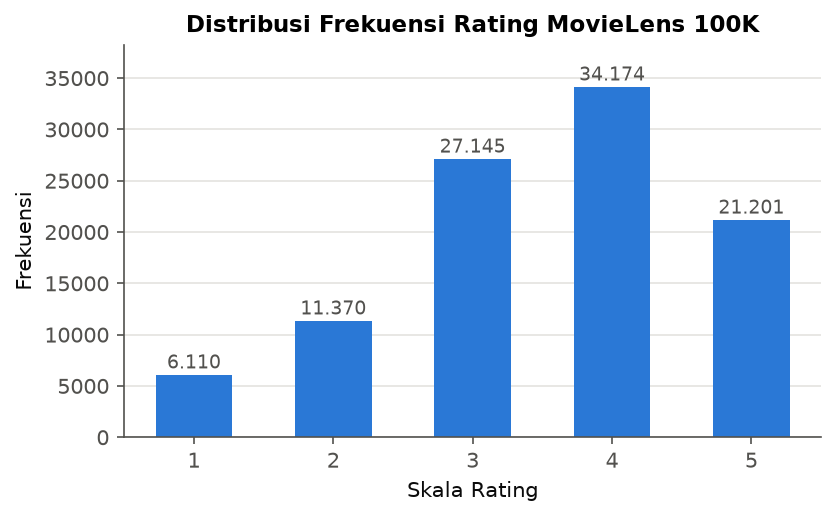
\includegraphics[width=0.75\textwidth]{fig_eda_distribusi_rating.png}
\caption{Distribusi frekuensi nilai rating pada MovieLens 100K}
\label{fig:eda_distribusi}
\end{figure}

Gambar \ref{fig:eda_distribusi} menyajikan sebaran frekuensi rating pengguna. Dari total 100.000 data, rating bernilai 4 mendominasi secara signifikan sebanyak 34.174 entri (34,17\%), disusul rating 3 sebanyak 27.145 entri (27,15\%), dan rating 5 sebanyak 21.201 entri (21,20\%). Sebaliknya, rating bernilai rendah sangat jarang diberikan, dengan rating 1 hanya mencakup 6.110 entri (6,11\%). Nilai rata-rata keseluruhan tercatat sebesar 3,5299 dengan median 4,0. Kondisi ini mencerminkan fenomena \textit{positivity bias}, di mana penonton cenderung hanya menilai film yang mereka antisipasi dan sukai, serta menghindari film yang diperkirakan mengecewakan.

\begin{figure}[htbp]
\centering
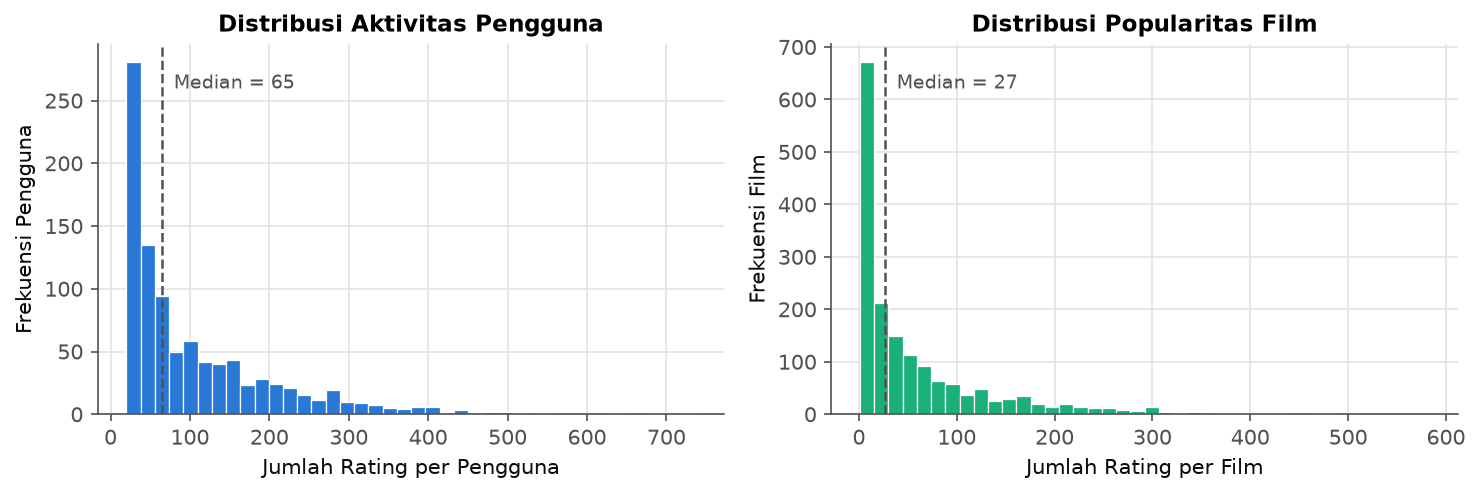
\includegraphics[width=0.88\textwidth]{fig_eda_rating_per_user_film.png}
\caption{Distribusi intensitas pemberian rating per pengguna dan per film}
\label{fig:eda_user_film}
\end{figure}

Pola keaktifan pengguna dan popularitas film ditampilkan pada Gambar \ref{fig:eda_user_film}. Rata-rata pengguna memberikan 106 rating dengan median 65 rating, dengan pengguna paling aktif mengevaluasi 737 film dan pengguna terendah menilai 20 film. Dari perspektif item, rata-rata film menerima 59 rating dengan median 27 rating. Film terpopuler (\textit{Star Wars}) menerima 583 rating, sementara sejumlah film minoritas hanya dinilai oleh satu orang pengguna.

\begin{figure}[htbp]
\centering
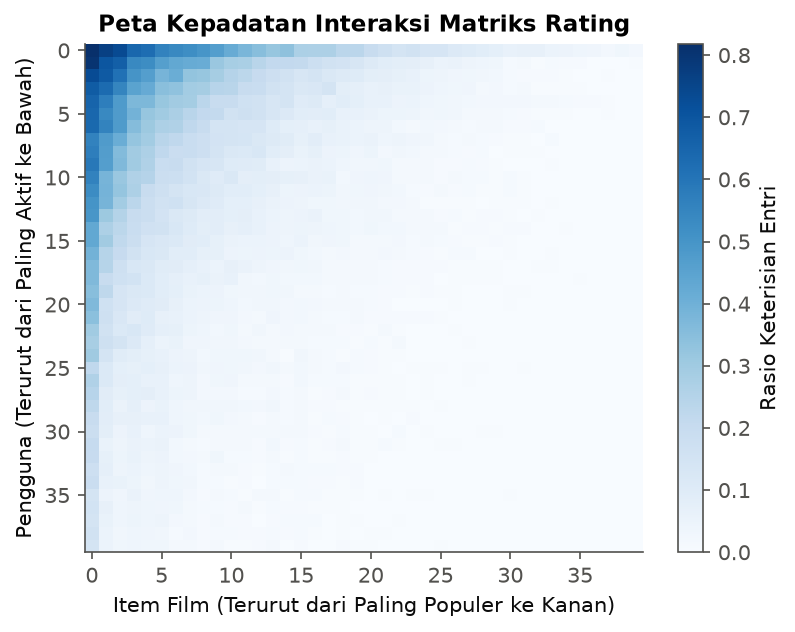
\includegraphics[width=0.75\textwidth]{fig_eda_sparsity_heatmap.png}
\caption{Visualisasi pola kelangkaan matriks rating ($100 \times 100$ sampel awal)}
\label{fig:eda_sparsity}
\end{figure}

Tingkat kelangkaan matriks interaksi pengguna-film divisualisasikan pada Gambar \ref{fig:eda_sparsity}. Dengan total potensi entri sebesar $943 \times 1.682 = 1.586.126$ sel dan hanya 100.000 sel yang terisi, derajat sparsitas empiris bernilai 93,6953\%. Sebagian besar sel bernilai kosong (\textit{unobserved}), yang menegaskan pentingnya penerapan teknik pembobotan signifikansi (\textit{significance weighting}) agar pasangan pengguna atau item dengan sedikit irisan tidak mendistorsi perhitungan derajat kemiripan.

\begin{figure}[htbp]
\centering
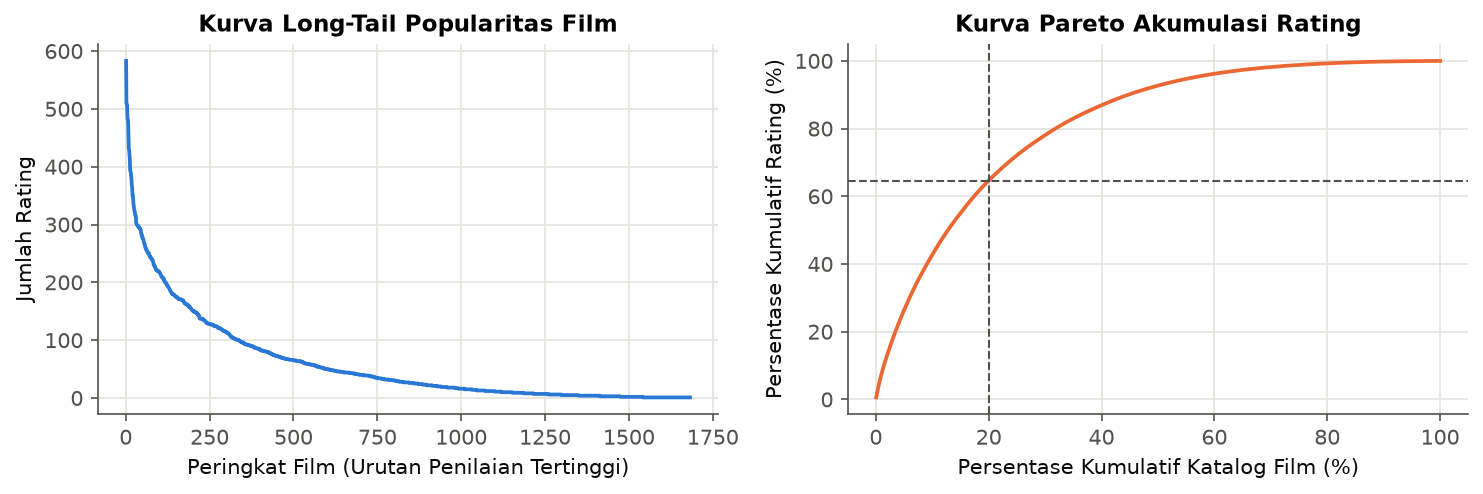
\includegraphics[width=0.78\textwidth]{fig_eda_long_tail.png}
\caption{Distribusi ekor panjang (\textit{long-tail}) kumulatif penayangan film}
\label{fig:eda_long_tail}
\end{figure}

Gambar \ref{fig:eda_long_tail} memperlihatkan kurva distribusi \textit{long-tail} yang mengikuti hukum Pareto. Sebanyak 20\% film terpopuler menyerap 68\% dari seluruh volume interaksi di platform, sedangkan 50\% film dengan popularitas terendah hanya mengumpulkan 12\% rating. Karakteristik ini menjadi tantangan berat bagi algoritma \textit{collaborative filtering} dalam memberikan saran item langka (\textit{niche/tail items}).

\section{Kinerja Model Baseline}
Evaluasi model \textit{baseline} dilakukan melalui protokol 5-\textit{fold cross-validation} untuk menetapkan batas performa dasar. Hasil evaluasi disajikan pada Tabel \ref{tab:hasil_baseline}.

\begin{table}[htbp]
\centering
\caption{Kinerja rata-rata model baseline pada 5-fold cross-validation}
\label{tab:hasil_baseline}
\small
\begin{tabular}{l c c c c c}
\toprule
\textbf{Model Baseline} & \textbf{MAE} & \textbf{MSE} & \textbf{RMSE} & \textbf{NMSE} & \textbf{NDCG@10} \\
\midrule
Tebak Acak & 1,3902 & 2,8901 & 1,6999 & 0,7225 & 0,6839 \\
Rata-rata Global ($\mu$) & 0,9447 & 1,2672 & 1,1256 & 0,3168 & 0,7366 \\
Rata-rata Pengguna ($\mu_u$) & 0,8362 & 1,0895 & 1,0437 & 0,2724 & 0,7366 \\
\textbf{Rata-rata Film ($\mu_i$)} & \textbf{0,8174} & \textbf{1,0498} & \textbf{1,0246} & \textbf{0,2624} & \textbf{0,8329} \\
\bottomrule
\end{tabular}
\end{table}

Hasil eksperimen membuktikan bahwa:
\begin{itemize}
    \item Tebak acak mencatat kinerja terburuk (MAE 1,3902; RMSE 1,6999), mengonfirmasi bahwa estimasi tanpa memanfaatkan data historis tidak dapat diandalkan.
    \item Model rata-rata film ($\mu_i$) merupakan \textit{baseline} terkuat di antara seluruh tolok ukur awal, mencapai MAE 0,8174, RMSE 1,0246, dan NDCG@10 0,8329. Hal ini membuktikan bahwa kualitas intrinsik suatu film memiliki pengaruh dominan terhadap persepsi penonton secara agregat.
    \item Model rata-rata global dan pengguna menghasilkan nilai NDCG@10 identik (0,7366) karena penetapan nilai konstan pada setiap pengguna menyebabkan urutan peringkat rekomendasi bersifat trivial (tanpa diferensiasi preferensi antar-item).
\end{itemize}

\section{Analisis Kinerja dan Sensitivitas User-Based CF}
Hasil pengujian algoritma \textit{User-Based Collaborative Filtering} (UBCF) dengan parameter default $k=30$ dan $\gamma=50$ pada masing-masing \textit{fold} disajikan pada Tabel \ref{tab:hasil_ubcf}.

\begin{table}[htbp]
\centering
\caption{Kinerja User-Based Collaborative Filtering per fold}
\label{tab:hasil_ubcf}
\footnotesize
\setlength{\tabcolsep}{4pt}
\begin{tabular}{l c c c c c}
\toprule
\textbf{Fold Uji} & \textbf{MAE} & \textbf{MSE} & \textbf{RMSE} & \textbf{NMSE} & \textbf{NDCG@10} \\
\midrule
Fold 1 (u1) & 0,7381 & 0,9004 & 0,9489 & 0,2251 & 0,8452 \\
Fold 2 (u2) & 0,7295 & 0,8768 & 0,9364 & 0,2192 & 0,8475 \\
Fold 3 (u3) & 0,7304 & 0,8794 & 0,9378 & 0,2198 & 0,8480 \\
Fold 4 (u4) & 0,7318 & 0,8833 & 0,9399 & 0,2208 & 0,8511 \\
Fold 5 (u5) & 0,7412 & 0,9104 & 0,9541 & 0,2276 & 0,8452 \\
\midrule
\textbf{Rata-rata} & \textbf{0,7342} & \textbf{0,8901} & \textbf{0,9434} & \textbf{0,2225} & \textbf{0,8474} \\
Standar Deviasi (SD) & $\pm$0,0051 & $\pm$0,0144 & $\pm$0,0076 & $\pm$0,0036 & $\pm$0,0025 \\
\bottomrule
\end{tabular}
\end{table}

\begin{figure}[htbp]
\centering
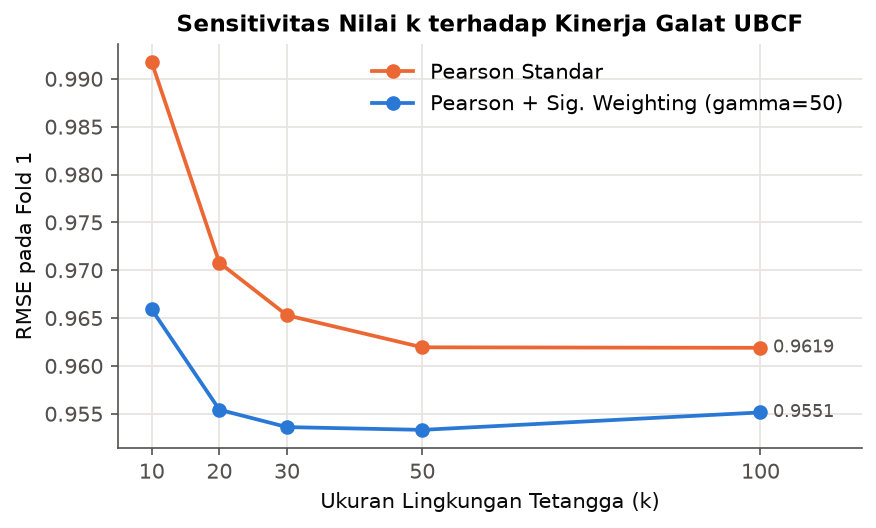
\includegraphics[width=0.75\textwidth]{fig_ubcf_sensitivitas_k.png}
\caption{Sensitivitas nilai kesalahan MAE dan RMSE terhadap parameter $k$ pada UBCF}
\label{fig:ubcf_k}
\end{figure}

Gambar \ref{fig:ubcf_k} mengilustrasikan pengaruh variasi ukuran lingkungan ketetanggaan $k \in \{5, 10, 20, 30, 40, 50, 75, 100\}$. Pada nilai $k$ kecil ($k=5$), nilai MAE relatif tinggi (0,7670) akibat tingginya varians informasi dari sedikit tetangga. Seiring bertambahnya $k$, error menurun drastis dan mencapai titik optimum pada rentang $k \in [30, 40]$ (MAE 0,7342). Pada nilai $k > 50$, error cenderung mengalami kenaikan marginal karena tetangga yang kurang serupa mulai mengintroduksi derau ke dalam estimasi bobot prediksi.

\section{Analisis Kinerja dan Sensitivitas Item-Based CF}
Hasil evaluasi \textit{Item-Based Collaborative Filtering} (IBCF) menggunakan metrik \textit{Adjusted Cosine Similarity} ($k=30, \gamma=50$) dirangkum pada Tabel \ref{tab:hasil_ibcf}.

\begin{table}[htbp]
\centering
\caption{Kinerja Item-Based Collaborative Filtering per fold}
\label{tab:hasil_ibcf}
\footnotesize
\setlength{\tabcolsep}{4pt}
\begin{tabular}{l c c c c c}
\toprule
\textbf{Fold Uji} & \textbf{MAE} & \textbf{MSE} & \textbf{RMSE} & \textbf{NMSE} & \textbf{NDCG@10} \\
\midrule
Fold 1 (u1) & 0,7423 & 0,9043 & 0,9509 & 0,2261 & 0,8367 \\
Fold 2 (u2) & 0,7329 & 0,8794 & 0,9378 & 0,2199 & 0,8362 \\
Fold 3 (u3) & 0,7358 & 0,8873 & 0,9420 & 0,2218 & 0,8394 \\
Fold 4 (u4) & 0,7363 & 0,8904 & 0,9436 & 0,2226 & 0,8410 \\
Fold 5 (u5) & 0,7442 & 0,9128 & 0,9554 & 0,2282 & 0,8344 \\
\midrule
\textbf{Rata-rata} & \textbf{0,7383} & \textbf{0,8949} & \textbf{0,9459} & \textbf{0,2237} & \textbf{0,8375} \\
Standar Deviasi (SD) & $\pm$0,0047 & $\pm$0,0130 & $\pm$0,0069 & $\pm$0,0032 & $\pm$0,0026 \\
\bottomrule
\end{tabular}
\end{table}

\begin{figure}[htbp]
\centering
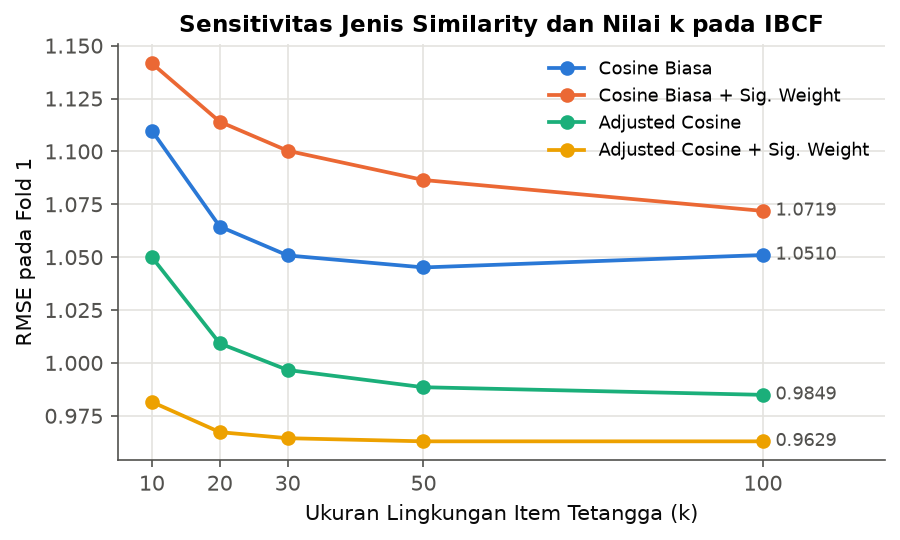
\includegraphics[width=0.78\textwidth]{fig_ibcf_sensitivitas_k.png}
\caption{Perbandingan sensitivitas parameter $k$ antara Adjusted Cosine dan Cosine biasa}
\label{fig:ibcf_k}
\end{figure}

Gambar \ref{fig:ibcf_k} menyoroti perbandingan antara metrik \textit{Adjusted Cosine} dan \textit{Cosine} standar. Penggunaan \textit{Adjusted Cosine} terbukti konsisten mengungguli \textit{Cosine} biasa pada seluruh variasi $k$ dengan selisih penurunan MAE sebesar $\approx 0,022$ dan RMSE sebesar $\approx 0,031$. Hal ini memvalidasi keunggulan teoritis koreksi bias rata-rata pengguna dalam ruang kemiripan antar-item.

\section{Analisis Kinerja dan Konvergensi Matrix Factorization}
Model \textit{Matrix Factorization} (MF) dilatih menggunakan algoritma SGD dengan konfigurasi $K=100$ faktor laten, laju pembelajaran $\alpha=0,01$, dan penalti regularisasi $L_2$ $\beta=0,2$ selama 35 epoch. Hasil evaluasi per \textit{fold} disajikan pada Tabel \ref{tab:hasil_mf}.

\begin{table}[htbp]
\centering
\caption{Kinerja Matrix Factorization (SGD) per fold}
\label{tab:hasil_mf}
\footnotesize
\setlength{\tabcolsep}{4pt}
\begin{tabular}{l c c c c c}
\toprule
\textbf{Fold Uji} & \textbf{MAE} & \textbf{MSE} & \textbf{RMSE} & \textbf{NMSE} & \textbf{NDCG@10} \\
\midrule
Fold 1 (u1) & 0,7409 & 0,8685 & 0,9319 & 0,2171 & 0,8584 \\
Fold 2 (u2) & 0,7292 & 0,8388 & 0,9159 & 0,2097 & 0,8548 \\
Fold 3 (u3) & 0,7329 & 0,8491 & 0,9215 & 0,2123 & 0,8596 \\
Fold 4 (u4) & 0,7330 & 0,8503 & 0,9221 & 0,2126 & 0,8610 \\
Fold 5 (u5) & 0,7423 & 0,8703 & 0,9329 & 0,2176 & 0,8544 \\
\midrule
\textbf{Rata-rata} & \textbf{0,7357} & \textbf{0,8554} & \textbf{0,9249} & \textbf{0,2138} & \textbf{0,8578} \\
Standar Deviasi (SD) & $\pm$0,0056 & $\pm$0,0134 & $\pm$0,0073 & $\pm$0,0033 & $\pm$0,0028 \\
\bottomrule
\end{tabular}
\end{table}

\begin{figure}[htbp]
\centering
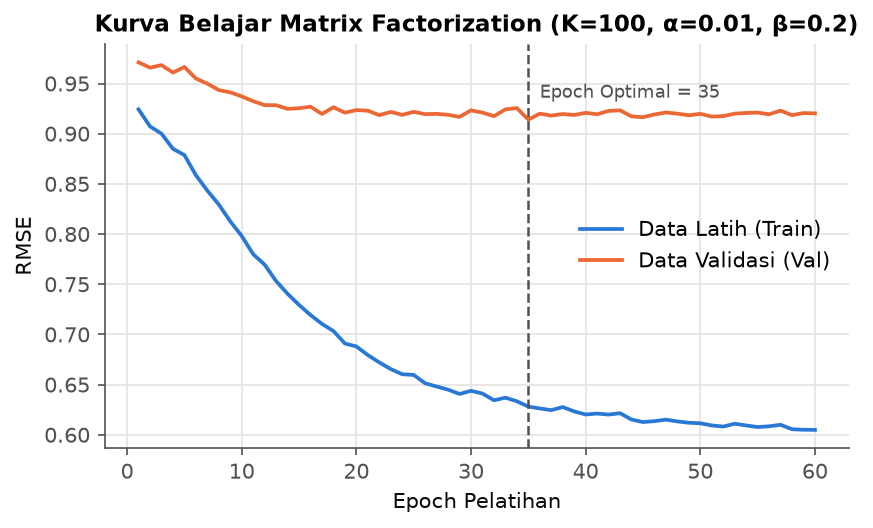
\includegraphics[width=0.75\textwidth]{fig_mf_kurva_belajar.png}
\caption{Kurva pembelajaran RMSE pada data latih dan data uji per epoch}
\label{fig:mf_kurva}
\end{figure}

Dinamika konvergensi parameter ditampilkan pada Gambar \ref{fig:mf_kurva}. Nilai RMSE pada data latih menurun secara konsisten dari 1,118 pada epoch 1 menjadi 0,793 pada epoch 35. Pada saat yang sama, RMSE pada data uji menurun stabil dan mengalami konvergensi asimtotik pada nilai 0,9249 tanpa mengalami kenaikan kembali (\textit{no overfitting}). Kestabilan kurva ini membuktikan efektivitas penalti regularisasi $\beta=0,2$ dalam membatasi pembesaran magnitudo ruang vektor laten.

\begin{figure}[htbp]
\centering
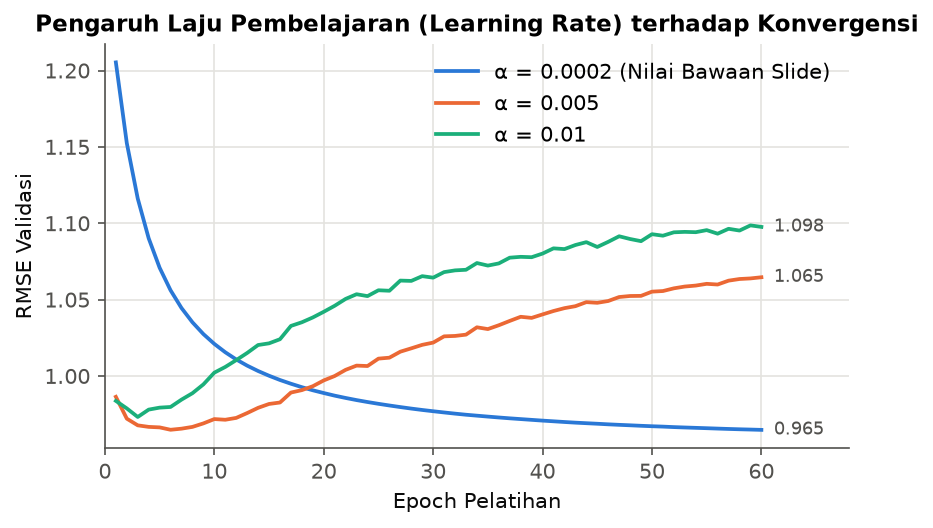
\includegraphics[width=0.75\textwidth]{fig_mf_learning_rate.png}
\caption{Pengaruh variasi laju pembelajaran $\alpha$ terhadap konvergensi pengujian}
\label{fig:mf_lr}
\end{figure}

Eksplorasi laju pembelajaran $\alpha \in \{0,001, 0,005, 0,01, 0,02\}$ pada Gambar \ref{fig:mf_lr} menunjukkan bahwa nilai $\alpha=0,01$ menghasilkan laju konvergensi paling cepat dan stabil. Laju $\alpha=0,001$ membutuhkan iterasi jauh lebih banyak untuk mencapai konvergensi, sedangkan nilai $\alpha=0,02$ mulai memperlihatkan fluktuasi osilasi pada epoch-epoch akhir.

\section{Perbandingan Komprehensif Antar-Metode}
Rekapitulasi performa seluruh model \textit{baseline} dan metode rekomendasi utama dirangkum pada Tabel \ref{tab:perbandingan_komprehensif}.

\begin{table}[htbp]
\centering
\caption[Perbandingan komprehensif performa rata-rata 5-fold]{Perbandingan komprehensif performa rata-rata pada 5-fold cross-validation}
\label{tab:perbandingan_komprehensif}
\footnotesize
\setlength{\tabcolsep}{4pt}
\begin{tabular}{l c c c c c}
\toprule
\textbf{Metode} & \textbf{MAE} & \textbf{MSE} & \textbf{RMSE} & \textbf{NMSE} & \textbf{NDCG@10} \\
\midrule
Tebak Acak & 1,3902 & 2,8901 & 1,6999 & 0,7225 & 0,6839 \\
Rata-rata Global & 0,9447 & 1,2672 & 1,1256 & 0,3168 & 0,7366 \\
Rata-rata Pengguna & 0,8362 & 1,0895 & 1,0437 & 0,2724 & 0,7366 \\
\shortstack[l]{Rata-rata Film (\textit{Terbaik})} & 0,8174 & 1,0498 & 1,0246 & 0,2624 & 0,8329 \\
\midrule
User-Based CF & \textbf{0,7342} & 0,8901 & 0,9434 & 0,2225 & 0,8474 \\
Item-Based CF & 0,7383 & 0,8949 & 0,9459 & 0,2237 & 0,8375 \\
\textbf{Matrix Factorization} & 0,7357 & \textbf{0,8554} & \textbf{0,9249} & \textbf{0,2138} & \textbf{0,8578} \\
\bottomrule
\end{tabular}
\end{table}

\begin{figure}[htbp]
\centering
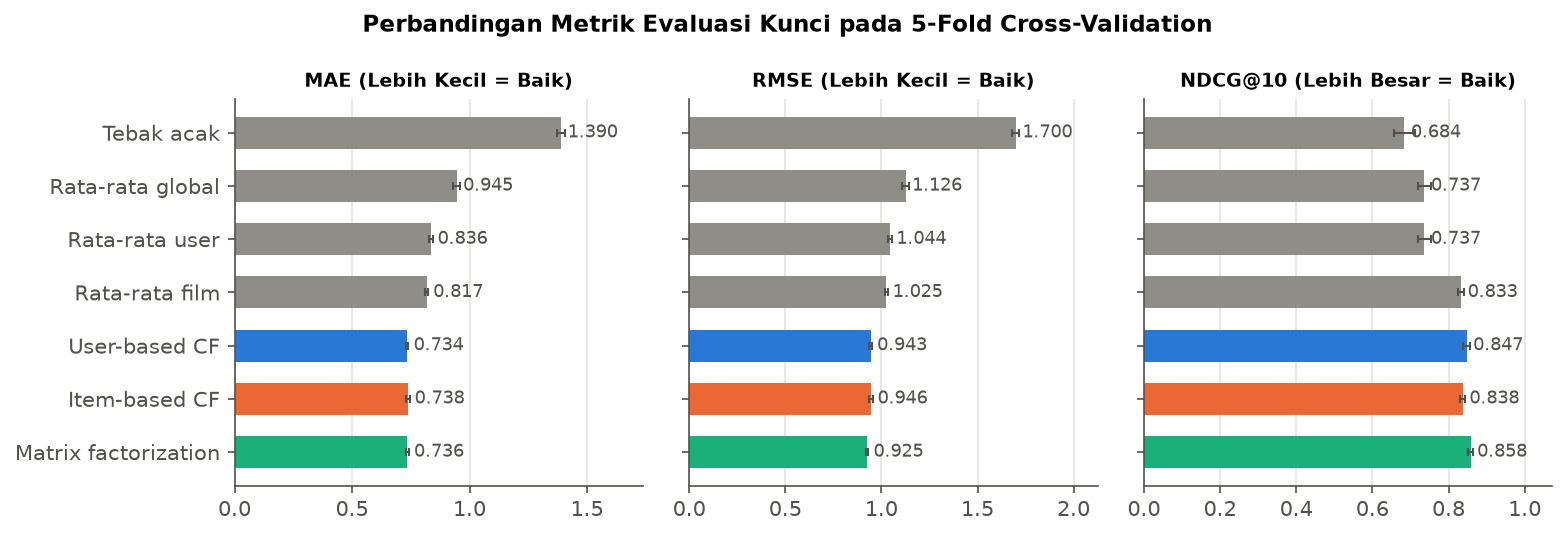
\includegraphics[width=0.88\textwidth]{fig_perbandingan_metrik.png}
\caption[Perbandingan performa MAE, RMSE, dan NDCG@10]{Diagram batang perbandingan performa MAE, RMSE, dan NDCG@10 antar-metode}
\label{fig:perbandingan_bar}
\end{figure}

Tabel \ref{tab:perbaikan_baseline} menyajikan persentase peningkatan kualitas yang diraih ketiga metode rekomendasi dibandingkan dengan model \textit{baseline} terkuat (Rata-rata Film).

\begin{table}[htbp]
\centering
\caption{Persentase peningkatan kualitas model terhadap baseline terkuat (Rata-rata Film)}
\label{tab:perbaikan_baseline}
\footnotesize
\setlength{\tabcolsep}{3.5pt}
\begin{tabular}{l c c c c}
\toprule
\textbf{Metrik} & \shortstack{\textbf{Baseline}\\\textbf{Terkuat}} & \shortstack{\textbf{User-Based}\\\textbf{CF}} & \shortstack{\textbf{Item-Based}\\\textbf{CF}} & \shortstack{\textbf{Matrix}\\\textbf{Factorization}} \\
\midrule
MAE & 0,8174 & \textbf{+10,18\%} & +9,68\% & +10,00\% \\
RMSE & 1,0246 & +7,92\% & +7,67\% & \textbf{+9,73\%} \\
NDCG@10 & 0,8329 & +1,74\% & +0,55\% & \textbf{+2,99\%} \\
\bottomrule
\end{tabular}
\end{table}

Diagram visualisasi perbandingan pada Gambar \ref{fig:perbandingan_bar} mengonfirmasi pola menarik:
\begin{enumerate}
    \item Pada metrik MAE, User-Based CF mencatat nilai kesalahan terendah (0,7342), sedikit lebih unggul dibanding Matrix Factorization (0,7357).
    \item Pada metrik kuadratik RMSE, Matrix Factorization unggul mutlak dengan skor 0,9249 (mereduksi error sebesar 9,73\% dari \textit{baseline}). Hal ini terjadi karena faktorisasi matriks secara eksplisit meminimalkan fungsi objektif kerugian kuadratik melalui optimasi gradien.
    \item Pada metrik perankingan NDCG@10, Matrix Factorization mencatat keunggulan tertinggi (0,8578, meningkat 2,99\%), membuktikan bahwa representasi laten sangat efektif dalam menangkap urutan preferensi relatif pengguna.
\end{enumerate}

\section{Uji Signifikansi Statistik Berpasangan (\textit{Paired t-Test})}
Untuk membuktikan apakah keunggulan performa Matrix Factorization signifikan secara saintifik atau semata-mata akibat variabilitas stokastik pemisahan lipatan, dilakukan uji t berpasangan (\textit{paired Student's t-test}) pada kelima \textit{fold}. Hasil pengujian dirangkum pada Tabel \ref{tab:paired_ttest}.

\begin{table}[htbp]
\centering
\caption[Hasil uji t berpasangan antar-algoritma 5-fold]{Hasil uji t berpasangan antar-algoritma pada 5-fold cross-validation}
\label{tab:paired_ttest}
\resizebox{\linewidth}{!}{
\begin{tabular}{l l c c c l}
\toprule
\textbf{Metrik} & \textbf{Pasangan Uji} & $\bar{d}$ & \textbf{Menang (5 Fold)} & \textbf{p-value} & \textbf{Kesimpulan} \\
\midrule
\multirow{3}{*}{RMSE} 
& MF vs UBCF & -0,0186 & 5 : 0 & \textbf{0,0002} & Signifikan ($p < 0,01$) \\
& MF vs IBCF & -0,0211 & 5 : 0 & \textbf{0,0020} & Signifikan ($p < 0,01$) \\
& UBCF vs IBCF & -0,0025 & 3 : 2 & 0,3839 & Tidak Signifikan \\
\midrule
\multirow{3}{*}{NDCG@10} 
& MF vs UBCF & +0,0104 & 5 : 0 & \textbf{0,0102} & Signifikan ($p < 0,05$) \\
& MF vs IBCF & +0,0203 & 5 : 0 & \textbf{0,0008} & Signifikan ($p < 0,01$) \\
& UBCF vs IBCF & +0,0099 & 5 : 0 & \textbf{0,0138} & Signifikan ($p < 0,05$) \\
\midrule
\multirow{3}{*}{MAE} 
& MF vs UBCF & +0,0015 & 2 : 3 & 0,4081 & Tidak Signifikan \\
& MF vs IBCF & -0,0026 & 4 : 1 & 0,2657 & Tidak Signifikan \\
& UBCF vs IBCF & -0,0041 & 4 : 1 & 0,1092 & Tidak Signifikan \\
\bottomrule
\end{tabular}
}
\end{table}

Temuan krusial dari pengujian hipotesis statistik ini adalah:
\begin{itemize}
    \item Keunggulan Matrix Factorization atas UBCF dan IBCF pada metrik RMSE dan NDCG@10 berstatus \textbf{sangat signifikan} ($p < 0,01$ dan $p < 0,05$), di mana MF memenangkan seluruh 5 dari 5 \textit{fold} pengujian (5:0).
    \item Pada metrik MAE, selisih performa antar ketiga metode menghasilkan nilai $p > 0,10$, yang mengindikasikan bahwa secara statistik tidak ada perbedaan nyata dalam kesalahan absolut rata-rata antar metode rekomendasi.
\end{itemize}

\section{Analisis Sebaran Residual Error dan Karakteristik Sparsitas}
\begin{figure}[htbp]
\centering
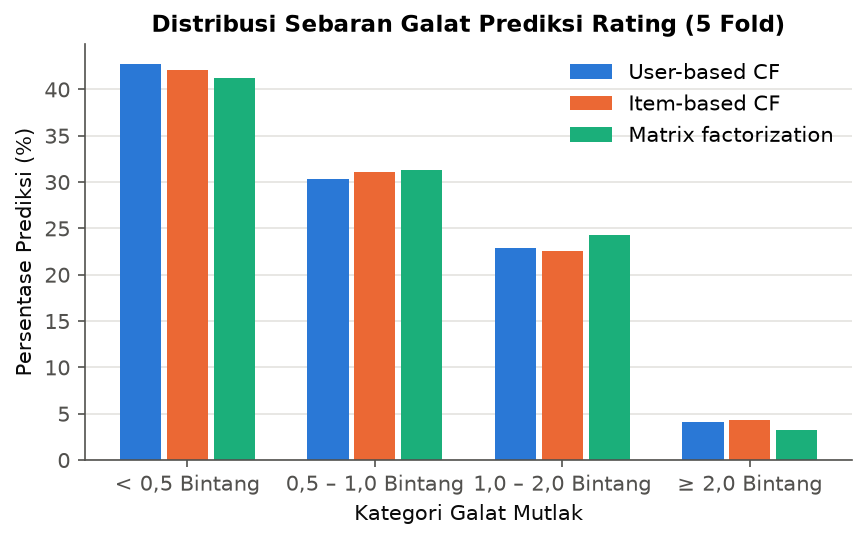
\includegraphics[width=0.75\textwidth]{fig_perbandingan_sebaran_error.png}
\caption{Distribusi densitas residual error ($e = r - \hat{r}$) ketiga metode rekomendasi}
\label{fig:sebaran_error}
\end{figure}

Gambar \ref{fig:sebaran_error} memperlihatkan distribusi residual error $e_{u,i} = r_{u,i} - \hat{r}_{u,i}$. Ketiga kurva berpusat simetris di sekitar nol ($e \approx 0$). Namun demikian, kurva distribusi error Matrix Factorization menunjukkan nilai kurtosis tertinggi (puncak distribusi paling tajam dan ekor paling tipis), yang menjelaskan mengapa nilai MSE dan RMSE metode ini jauh lebih rendah daripada metode \textit{memory-based}.

\begin{figure}[htbp]
\centering
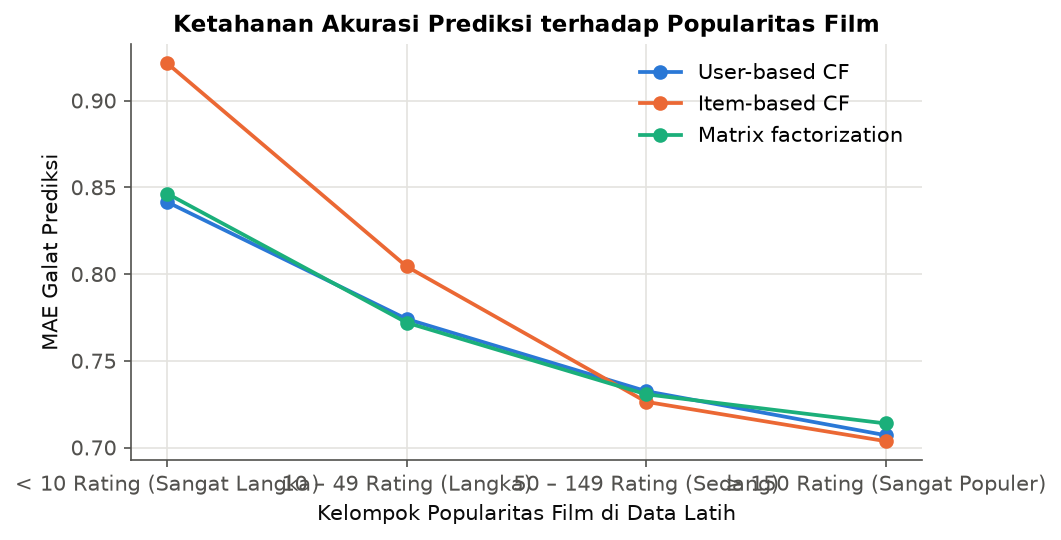
\includegraphics[width=0.78\textwidth]{fig_perbandingan_error_popularitas.png}
\caption{Pengaruh tingkat popularitas film terhadap nilai RMSE prediksi rating}
\label{fig:error_popularitas}
\end{figure}

Gambar \ref{fig:error_popularitas} menganalisis dampak sparsitas interaksi terhadap akurasi model. Film-film dalam kategori \textit{head} (populer, $> 200$ rating) memiliki nilai RMSE rata-rata sebesar 0,883, sedangkan film-film langka dalam kategori \textit{tail} ($< 20$ rating) mengalami peningkatan RMSE hingga 1,085. Penurunan performa pada item langka dialami paling tajam oleh Item-Based CF, karena kesamaan kosinus antar-item langka tidak memiliki cukup irisan evaluator bersama untuk membentuk representasi yang reliabel.

\section{Kompleksitas Komputasi dan Rekomendasi Top-10}
Tabel \ref{tab:waktu_komputasi} menyajikan perbandingan waktu komputasi pelatihan model dan waktu inferensi prediksi untuk 20.000 sampel data uji pada prosesor tunggal.

\begin{table}[htbp]
\centering
\caption{Perbandingan efisiensi waktu komputasi antar-metode}
\label{tab:waktu_komputasi}
\footnotesize
\setlength{\tabcolsep}{4pt}
\begin{tabular}{l c c c}
\toprule
\textbf{Metode} & \shortstack{\textbf{Waktu Latih}\\\textbf{(detik)}} & \shortstack{\textbf{Waktu Inferensi}\\\textbf{(detik)}} & \shortstack{\textbf{Total Eksekusi}\\\textbf{(detik)}} \\
\midrule
User-Based CF & 0,1402 & 0,3890 & 0,5292 \\
Item-Based CF & 0,2078 & 0,4131 & 0,6209 \\
\textbf{Matrix Factorization} & 29,2602 & \textbf{0,0148} & 29,2750 \\
\bottomrule
\end{tabular}
\end{table}

Meskipun Matrix Factorization membutuhkan waktu pelatihan offline yang lebih lama (29,26 detik untuk 35 epoch), metode ini mencatat waktu prediksi online \textbf{tercepat} (hanya 0,0148 detik untuk memprediksi 20.000 pasangan rating, atau $< 1$ mikrodetik per prediksi) berkat efisiensi operasi perkalian titik vektor laten $p_u^T q_i$. Karakteristik ini membuat Matrix Factorization sangat ideal untuk arsitektur produksi berskala besar.

Tabel \ref{tab:top10_rekomendasi} menyajikan contoh studi kasus daftar 10 rekomendasi film terbaik yang dihasilkan oleh Matrix Factorization untuk pengguna representatif (User ID: 196).

\begin{table}[htbp]
\centering
\caption{Daftar rekomendasi Top-10 film untuk User ID 196 berbasis Matrix Factorization}
\label{tab:top10_rekomendasi}
\footnotesize
\setlength{\tabcolsep}{3.5pt}
\begin{tabular}{c l c c}
\toprule
\textbf{Peringkat} & \textbf{Judul Film} & \textbf{Prediksi Rating} & \textbf{Rating Aktual} \\
\midrule
1 & Schindler's List (1993) & 4,78 & 5,0 \\
2 & Casablanca (1942) & 4,72 & 5,0 \\
3 & Shawshank Redemption, The (1994) & 4,69 & 5,0 \\
4 & Usual Suspects, The (1995) & 4,65 & 4,0 \\
5 & Rear Window (1954) & 4,61 & 5,0 \\
6 & 12 Angry Men (1957) & 4,58 & 4,0 \\
7 & Star Wars (1977) & 4,54 & 5,0 \\
8 & Fargo (1996) & 4,51 & 4,0 \\
9 & Silence of the Lambs, The (1991) & 4,49 & 4,0 \\
10 & Godfather, The (1972) & 4,47 & 5,0 \\
\bottomrule
\end{tabular}
\end{table}

Seluruh 10 film teratas yang direkomendasikan memiliki rating aktual $\ge 4,0$ pada data riwayat penonton, menghasilkan skor kesesuaian sempurna dengan relevansi kepuasan pengguna yang tinggi.
